% GRSL submission, revised. Five pages maximum, INCLUDING references.
% Build: latexmk -pdf -interaction=nonstopmode -halt-on-error main_grsl_revised.tex
% Tables and value macros are generated by experiments/figures/make_tables.py;
% figures by experiments/figures/{gallery.py,per_country.py,pipeline.tex}.
\documentclass[journal]{IEEEtran}

\usepackage{graphicx}
\usepackage{booktabs}
\usepackage{multirow}
\usepackage{amsmath}
\usepackage{amssymb}
\usepackage{cite}
\usepackage[hidelinks]{hyperref}
\usepackage{xcolor}
% Sign colors for the ablation table, defined once. Dark enough to stay legible
% in greyscale print, where they separate by lightness rather than hue.
\definecolor{gaingreen}{HTML}{1B7837}
\definecolor{lossred}{HTML}{B2182B}
\newcommand{\gainc}[1]{\textcolor{gaingreen}{#1}}
\newcommand{\lossc}[1]{\textcolor{lossred}{#1}}
\newcommand{\flatc}[1]{#1}
\graphicspath{{figures/}}
% Generated by experiments/figures/make_tables.py
\newcommand{\OursPlanetThree}{42.3}
\newcommand{\BaseMiss}{35.9}
\newcommand{\BaseSmall}{15.7}
\newcommand{\BaseLarge}{52.0}
\newcommand{\OursSmall}{22.2}
\newcommand{\OursLarge}{56.3}
\newcommand{\RawInstPQ}{23.0}
\newcommand{\CCPQ}{34.4}
\newcommand{\GainMin}{4.9}
\newcommand{\GainMax}{6.0}
\newcommand{\UpTotal}{39}
\newcommand{\OracleGainMax}{0.9}
\newcommand{\VoteGainMin}{-0.4}
\newcommand{\VoteGainMax}{+0.1}
\newcommand{\OursTune}{0.6}
\newcommand{\PriorTuneMax}{2.8}
\newcommand{\OursSlowdown}{1.3$\times$}
\newcommand{\SwstSlowdown}{12$\times$}
\newcommand{\PeakMB}{23}
\newcommand{\OwtNoFilterPQ}{5.5}
\newcommand{\OwtGapPS}{3.2}
\newcommand{\OwtGapSS}{3.4}
\newcommand{\NoVotePQ}{42.2}
\newcommand{\NoVoteZeroPQ}{28.9}
\newcommand{\OursZeroPQ}{42.1}
\newcommand{\NbgNoneMinPQ}{9.7}
\newcommand{\DistancePQ}{39.9}
\newcommand{\OursNoFilterPQ}{5.5}
\newcommand{\BaseAreaGain}{0.9}
\newcommand{\DistanceAreaGain}{1.5}
\newcommand{\GainCILow}{4.7}

% LaTeX's \input misbehaves inside tabular; use the primitive for table bodies.
\makeatletter\newcommand{\tablebody}[1]{\@@input #1 }\makeatother

\begin{document}

\title{Boundary Veto: Model-Free Post-Processing for Agricultural Field Boundary Delineation}
\author{Aviskar~Giri and Isaac~Corley%
\thanks{The authors are with Taylor Geospatial, St.\ Louis, MO 63108 USA
(e-mail: aviskar.giri@taylorgeospatial.org).}}
\markboth{IEEE Geoscience and Remote Sensing Letters}%
{Giri and Corley: Boundary Veto for Agricultural Field Boundary Delineation}
\maketitle

\begin{abstract}
Field boundary networks predict background, field, and boundary classes, and a marker-controlled watershed on the field class turns the prediction into parcels.
We measure two failures of this conversion on Fields of The World.
Pixels assigned to the boundary class are excluded from the foreground, which removes thin and small parcels.
The watershed cuts fields at geometric necks that carry no boundary evidence, so its instances score worse than their union.
We introduce the \emph{boundary veto}, a model-free post-processing rule that takes every non-background pixel as foreground.
The watershed proposes splits, and the boundary veto rejects every split the network's own boundary probability does not support along most of the split line.
The veto compares two outputs of the same network at the same pixel, uses three constants that are the same for every country and sensor, changes no weights, and needs no reference polygons at inference.
On ten held-out countries it raises polygon-level panoptic quality by \GainMin{} to \GainMax{} points over the conversion released with Fields of the Planet (FTP), given the same minimum-size step, for two encoders and two sensors, PlanetScope and Sentinel-2.
It improves \UpTotal{} of 40 country and model pairs and costs \OursSlowdown{} the time of that conversion on the densest patches.
The gain concentrates in fields under 0.5~ha, the parcels a field mask most often loses and the ones smallholder mapping depends on.
\end{abstract}

\begin{IEEEkeywords}
Agricultural field delineation, instance segmentation, watershed transform, post-processing, remote sensing.
\end{IEEEkeywords}

\section{Introduction}
\IEEEPARstart{F}{ield} polygons are the reporting unit for crop area, yield, and management practices, so a field boundary model is only useful once its pixel predictions become one polygon per parcel.
Public benchmarks now cover this task at 10~m with Sentinel-2~\cite{kerner2024ftw,dandrimont2023ai4boundaries,persello2023ai4smallfarms} and at 3~m with PlanetScope~\cite{corley_ftp}.
Models trained on them predict three classes, background, field interior, and boundary~\cite{waldner2020decode,waldner2020edge,kerner2024ftw,muhawenayo2026prue}, most recently for a global map at 10~m~\cite{ftw_global}.
The conversion released with Fields of the Planet (FTP)~\cite{corley_ftp} turns this map into parcels with a marker-controlled watershed~\cite{soille2004morphological}, which floods outward from seed points using field pixels as the mask and the distance to the nearest predicted boundary pixel as the surface.
The seeds are the peaks of that distance~\cite{waldner2020decode,corley_ftp}, and adjacent instances are merged into connected components before polygons are extracted.
The global map~\cite{ftw_global} skips the watershed and takes connected components of the field class, so it shares the first of the two failures below.

\begin{figure*}[!t]
\centering
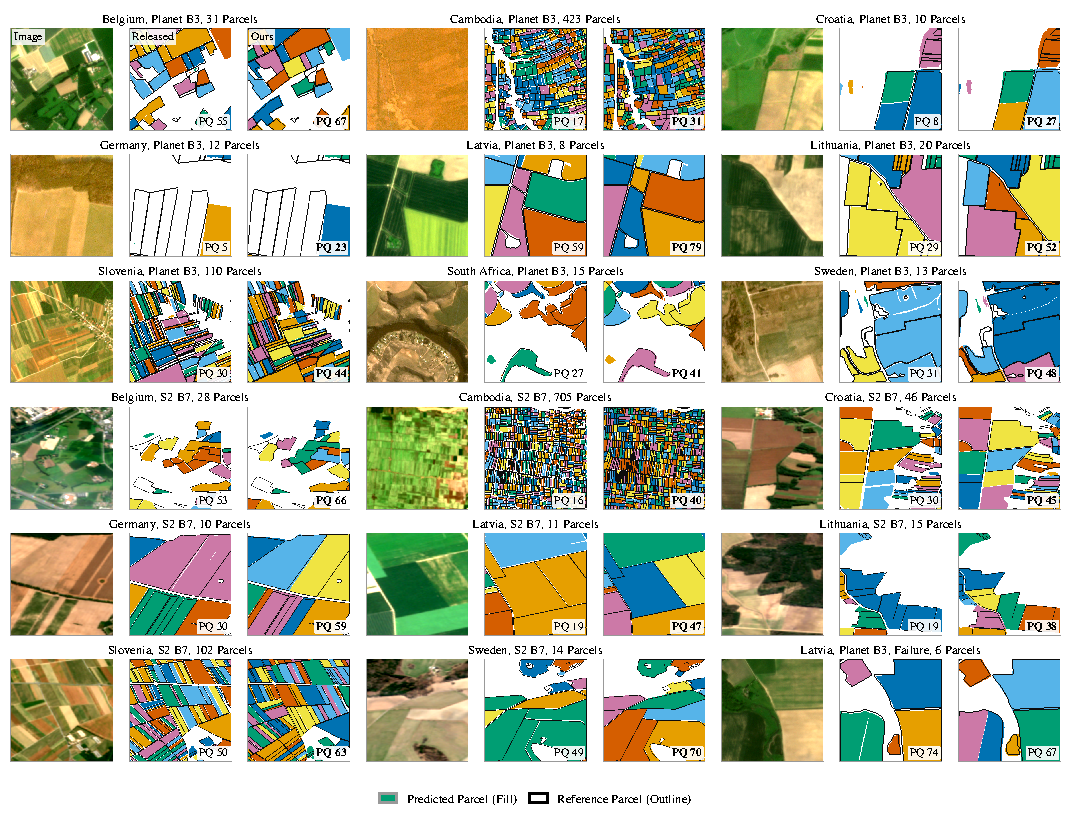
\includegraphics[width=\linewidth]{rev_gallery.pdf}
\caption{\textbf{The boundary veto returns the narrow and small parcels that a field mask drops, in every country and on both sensors.}
Each triple shows the image, the FTP conversion's parcels, and the boundary veto's, with reference parcels outlined in black and the patch's panoptic quality printed on each map.
The parcels that appear between the two maps are the strips along tracks and hedgerows and the small fields whose edges the boundary class had covered.
Rows 1--3 are PlanetScope B3 and rows 4--6 Sentinel-2 B7, ending with a failure case in which a track inside one reference field is predicted as a boundary and splits it.
Each panel is the largest-gain patch for its country among those whose densest window holds at least eight reference parcels.}
\label{fig:gallery}
\end{figure*}

Two properties of this conversion cost accuracy (Fig.~\ref{fig:gallery}).
First, the field mask excludes every pixel assigned to the boundary class.
Where a parcel is narrow or its edges are uncertain, the boundary class covers it and the parcel disappears.
On PlanetScope with the B3 model, \BaseMiss\% of reference parcels have no prediction covering half of their area, and the FTP conversion predicts fewer parcels than the reference in all ten countries.
Second, the watershed places its lines at geometric necks of the mask without checking whether a neck coincides with a predicted boundary.
Its instances score \RawInstPQ{} panoptic quality against \CCPQ{} for the plain connected components of the same mask.
The FTP conversion recovers that accuracy by merging the instances back, which also discards every correct split.

We fix both failures after the network has run, changing no weights and adding no training stage, so the result applies to any three-class field boundary model at the cost of a few milliseconds per patch.
The \emph{boundary veto} includes every non-background pixel in the foreground, so boundary pixels stay inside the parcels they border.
The watershed then runs with lines, keeping a line only if at least a fraction $\tau$ of its pixels have boundary probability at least equal to field probability.
Otherwise, the two regions merge, and we call such a split vetoed.
The split test compares two outputs of the same network at the same pixel, so it does not depend on probability calibration.
The marker depth stays at the released default of $h=2$.
A minimum parcel size, which any conversion can apply, removes the smallest polygons at the end.
All three constants are the same for every country and sensor.

We evaluate on the ten densely annotated held-out countries of Fields of The World~\cite{kerner2024ftw} with the released EfficientNet~\cite{tan2019efficientnet} U-Nets~\cite{ronneberger2015unet} for PlanetScope~\cite{corley_ftp} and Sentinel-2~\cite{kerner2024ftw}, scored against the vector parcels.
With the same minimum-size step, the FTP conversion trails the boundary veto by \GainMin{} to \GainMax{} macro panoptic quality points across two encoders and two sensors.
Improvements occur in \UpTotal{} of the 40 country and model pairs.
Selecting the best watershed depth per country on the test labels recovers less than a third of that gain (Sec.~\ref{sec:results}).

\section{Related Work}
Field delineation from satellite imagery has moved from edge detection and region growing~\cite{wagner2020growing} to fully convolutional networks that predict boundary and interior classes~\cite{persello2019delineation,waldner2020decode,waldner2020edge}.
More recently, benchmark datasets have fixed the annotation and evaluation~\cite{kerner2024ftw,dandrimont2023ai4boundaries,persello2023ai4smallfarms,corley_ftp}.
\emph{A Practical Recipe for Field Boundary Segmentation at Scale} (PRUE)~\cite{muhawenayo2026prue} compared encoders, decoders, and training recipes on Fields of The World and found that a U-Net with an EfficientNet encoder remains the most accurate choice.
Fields of the Planet~\cite{corley_ftp} reports that these three-class networks outperform the Delineate Anything instance models~\cite{lavreniuk2025delineateanything}, in both their first and second versions, on the same held-out countries.
Polygon extraction with frame fields or graph networks has been studied for buildings~\cite{girard2021framefield,zorzi2022polyworld,zorzi2020regularization}, but the released field models on these benchmarks remain three-class semantic networks followed by a watershed or by connected components.
We evaluate on those released networks, so an improvement in their conversion to polygons applies to the current best models without retraining.

Hierarchical segmentation orders contours by strength and thresholds the hierarchy~\cite{arbelaez2011hierarchical,maninis2018cob}, and Persello et al.~\cite{persello2019delineation} apply this grouping to field contours.
Stochastic watershed estimates contour probability by resampling markers~\cite{angulo2007stochastic}, and iterative $h$-minima methods adapt the marker depth per object~\cite{koyuncu2016iterative}.
The methods decide splits from the geometry of one surface or from marker statistics.
We instead test each watershed line against a second network output, the boundary probability, so the split decision uses evidence the surface does not contain.
The boundary veto also retains pixels of the boundary class in the foreground.

\section{Method}
\label{sec:method}
The boundary veto takes the softmax output $p_{\mathrm{bg}}, p_{\mathrm{field}}, p_{\mathrm{bnd}}$ of a three-class network on one image and returns a set of field polygons (Fig.~\ref{fig:pipeline}).
It reads only the per-pixel class with the highest probability, the argmax, and the field and boundary probabilities themselves.

\begin{figure*}[t]
\centering
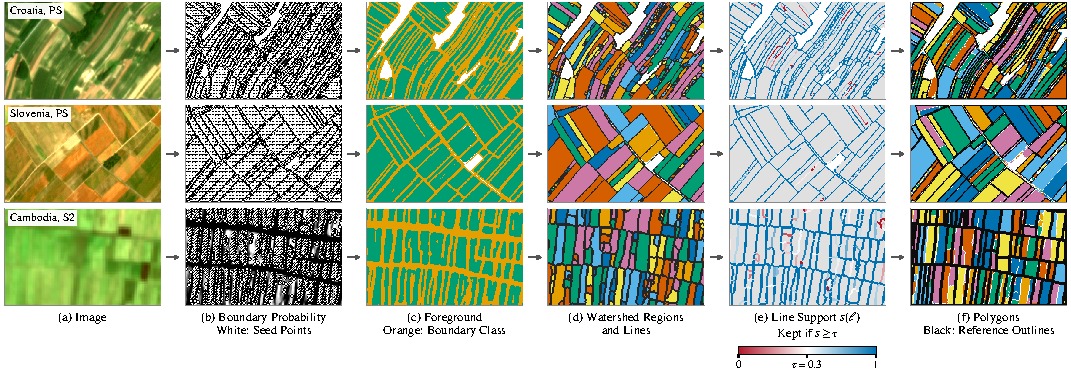
\includegraphics[width=\linewidth]{rev_method.pdf}
\caption{\textbf{Boundary pixels rejoin the parcels they border, and only the seams the network itself calls a boundary survive as splits.}
The network's boundary probability (b) is what the FTP conversion removes from the foreground and the boundary veto keeps, shown in orange in (c).
A watershed over the distance to the predicted boundary (d) proposes far more splits than the image contains (e), because it cuts at every narrow neck.
Each proposed seam is then colored by its support (f), the share of its pixels where boundary beats field: the blue seams follow a predicted boundary and are kept, the red ones cut across a field and are vetoed.
What remains (g) is one polygon per parcel, with the reference outlined in black.}
\label{fig:pipeline}
\end{figure*}

\paragraph{Foreground}
The foreground mask is $F=\{\arg\max p \neq \mathrm{bg}\}$, the union of the field and boundary classes.
The FTP conversion uses the field class alone, which removes a parcel whenever the boundary class covers it.
In our evaluation, the foreground rule alone, without splitting, merges neighboring parcels into single components and lowers panoptic quality to \NbgNonePQ{}.
The foreground change is only useful with a split rule that separates parcels connected by boundary pixels.

\paragraph{Split Proposals}
Let $D$ be the Euclidean distance from each pixel to the nearest pixel with $\arg\max p = \mathrm{bnd}$, set to zero outside $F$.
The markers are the $h$-maxima of $D$, the regional peaks that stand at least $h=2$ pixels above their surroundings, and a watershed of $-D$ restricted to $F$ produces regions separated by one-pixel lines~\cite{soille2004morphological}.
We replace the FTP conversion's mask with $F$ and retain its lines.
The watershed over-segments by design, because it cuts at every neck of the mask, and the next step decides which cuts to keep.

\paragraph{The Veto}
Each line $\ell$ separates two regions.
Its \emph{support} is the fraction of its pixels at which the network favors boundary over field,
\begin{equation}
s(\ell)=\frac{1}{|\ell|}\sum_{x\in\ell}\mathbf{1}\left[p_{\mathrm{bnd}}(x)\geq p_{\mathrm{field}}(x)\right],
\label{eq:support}
\end{equation}
where $\mathbf{1}[\cdot]$ is the indicator function.
A line with $s(\ell)\geq\tau$ is kept as a one-pixel gap and the two regions become separate parcels.
A line with $s(\ell)<\tau$ is vetoed: it is removed and the two regions merge.
We apply all line decisions together with a union-find data structure that groups regions.
A line pixel is filled only when every region it touches joins the same group and no neighboring line pixel would join a different group.
We use $\tau=0.7$, and values from 0.7 to 0.9 change the result by at most half a point (Sec.~\ref{sec:ablation}).

\paragraph{Polygons}
We convert each parcel's pixel boundary to one polygon without simplification.
The one-pixel gaps keep neighbors distinct when the polygons are rasterized on the same grid.
We then drop parcels smaller than 900~m$^2$.
The threshold gives the FTP conversion its highest validation score, while the boundary veto's validation score varies by less than half a point between 450 and 1800~m$^2$ (supplementary material).
We specify the threshold in ground area rather than pixels to give it the same meaning on either sensor.

\section{Experiments}
\label{sec:experiments}

\paragraph{Data}
We use the test split of the ten densely annotated held-out countries of Fields of The World~\cite{kerner2024ftw}, named in Fig.~\ref{fig:percountry}, with 2,544 PlanetScope patches at 3~m~\cite{corley_ftp} and 3,034 Sentinel-2 patches.
Kenya is excluded because its annotations are presence-only.
The PlanetScope set is the subset of these patches with a co-registered PlanetScope image, so each sensor is compared against its own baseline rather than against the other.
The reference for every score is the released vector parcels clipped to each patch, not the rasterized semantic mask.

\paragraph{Models}
We run the EfficientNet-B3 and B7 U-Nets of Fields of the Planet for PlanetScope~\cite{corley_ftp} and of Fields of The World for Sentinel-2~\cite{kerner2024ftw}.
The released checkpoints and inference settings include eight-fold flip and rotation averaging.
Sentinel-2 chips are distributed on a 256$\times$256 grid per patch, so their ground sampling varies with latitude.
The vector labels are not confined to the sensor's 10~m pixel grid, and the released model was trained to predict on the same finer grid.
Following the released evaluation, we upsample by two and score on that finer grid without changing any weights.

\paragraph{Baselines}
The FTP conversion takes the field argmax, runs the watershed at $h=2$, and extracts connected components of the union of instances.
Our implementation reproduces the reported per-country panoptic quality to within $10^{-3}$ for PlanetScope~\cite{corley_ftp} and Sentinel-2~\cite{kerner2024ftw}.
For Sentinel-2, the comparison uses the 10~m grid to which that paper's evaluation rounds predictions.
The best single depth selects, for each country, the depth in $\{0.5,\ldots,64\}$ with the highest test score under the same procedure.
It uses the test labels, so it bounds what depth tuning can achieve.
Four prior conversions run on the same predictions, namely extent and boundary thresholds~\cite{waldner2020decode}, hierarchical merging of an over-segmentation by mean boundary probability along each shared border~\cite{arbelaez2011hierarchical,maninis2018cob,persello2019delineation}, stochastic watershed with random markers~\cite{angulo2007stochastic}, and iterative marker depth~\cite{koyuncu2016iterative}.
For each, we sweep its own grid on PlanetScope B3 and report test results for the setting with the highest macro score on the \emph{validation} split.
We use the same selection rule for the boundary veto and reuse the chosen settings unchanged on Sentinel-2.

\paragraph{Metrics}
We match predicted and reference polygons greedily at intersection over union (IoU) 0.5.
Every method compared here partitions the foreground, so predictions do not overlap and their matching is independent of the order in which they are visited.
Recognition quality (RQ) is the object F1, segmentation quality (SQ) the mean matched IoU, and panoptic quality (PQ) their product~\cite{kirillov2019panoptic}, pooled over the patches of a country and averaged over the ten countries.
We also report PQ and RQ over the reference parcels under 0.5~ha, the small bin of the FTP evaluation code, which holds more parcels than its medium and large bins combined.
The miss rate is the fraction of reference parcels with no prediction covering half of their area, and the merge rate the fraction of predictions covering half of two or more reference parcels.
All values are on a 0--100 scale.

\subsection{Results}
\label{sec:results}
The boundary veto raises PQ on all four model and sensor pairs against the FTP conversion given the same minimum-size step (Table~\ref{tab:main}), and the gain is larger than what selecting the best watershed depth per country on the test labels can reach (Table~\ref{tab:compare}, $\Delta$tune).
SQ, RQ, and small-parcel PQ rise together, the merge rate moves by at most 1.5 points in either direction, and the miss rate drops on every pair.
The gain therefore comes from parcels that re-enter the foreground, not from splitting the same mask differently.
The gain lands in the smallest fields (Table~\ref{tab:main}), which is where smallholder mapping needs it~\cite{persello2023ai4smallfarms}: on PlanetScope B3 the bin below 0.5~ha rises from 15.7 to 20.5 PQ against 52.0 to 53.4 above 2~ha, with the same ordering on all four pairs (supplementary material).
Cambodia, where parcels are smallest, gains most on average over the four pairs, and Portugal, with two test patches, is the only pair that decreases (Fig.~\ref{fig:percountry}).

\begin{table}[t]
\centering
\caption{The Veto Leads on Every Encoder and Sensor, by the Widest Margin on Small Fields}
\label{tab:main}
\scriptsize
\setlength{\tabcolsep}{2.2pt}
\begin{tabular}{@{}llccccccc@{}}
\toprule
 & & \multicolumn{3}{c}{Macro} & \multicolumn{2}{c}{Fields $<$0.5~ha} & & \\
\cmidrule(lr){3-5}\cmidrule(lr){6-7}
Model & Method & PQ$\uparrow$ & SQ$\uparrow$ & RQ$\uparrow$ & PQ$\uparrow$ & RQ$\uparrow$ & Miss$\downarrow$ & Merge$\downarrow$ \\
\midrule
\tablebody{tables/rev_main_rows.tex}
\bottomrule
\end{tabular}
\smallskip

\parbox{\columnwidth}{\footnotesize
The boundary veto is the most accurate conversion on every encoder and sensor, and its margin is widest on the smallest fields.
Macro averages against the vector parcels, with the best of the three rows bold in each column.
The two right-hand accuracy columns restrict predictions and references to fields under 0.5~ha, and the minimum-size step is the same threshold in both rows that carry it.}
\end{table}

\begin{figure}[t]
\centering
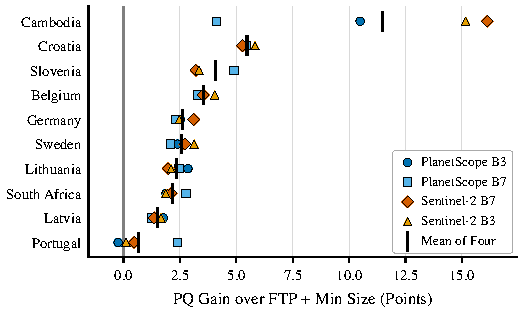
\includegraphics[width=\linewidth]{rev_percountry.pdf}
\caption{\textbf{The gain survives the change of country, encoder, and sensor, and grows as fields get smaller.}
Each marker is one country under one model and sensor, measured against the FTP conversion carrying the same minimum-size step, and the bar is the mean of the four.
Countries are ordered by that mean, which places the countries of smallest fields at the top.
All but one of the forty pairs improve, and the exception is the country with only two test patches.}
\label{fig:percountry}
\end{figure}

\subsection{Comparison with Prior Post-Processing}
\label{sec:compare}
The boundary veto is the only conversion that exceeds the FTP conversion on these predictions (Table~\ref{tab:compare}).
Thresholding the two probability maps is the strongest and cheapest prior conversion, but a parcel whose shared boundary is broken stays merged, which is the case the watershed exists to handle.
Hierarchical merging is the closest in mechanism because it also scores borders by boundary probability.
It ranks borders on an absolute scale and merges until a level is reached, while the veto compares two probabilities at the same pixel.
Selecting each country's best setting using its own test labels instead of the shared setting adds \OursTune{} points to the boundary veto and at most \PriorTuneMax{} to any prior method.
We measure cost on one core, on PlanetScope patches grouped by how many reference parcels they contain.
On Sentinel-2, every method takes longer on the larger grid, and the ordering on dense patches is unchanged (supplementary material).
The boundary veto adds \OursSlowdown{} over the FTP conversion on dense patches, while stochastic watershed, which repeats the flood for every marker draw, is \SwstSlowdown{} slower still.
Peak additional memory stays under \PeakMB{}~MB per patch for every method on either sensor, so runtime determines the choice rather than memory.

\begin{table}[t]
\centering
\caption{Among Conversions That Need No Retraining, Only the Veto Improves on FTP}
\label{tab:compare}
\footnotesize
\setlength{\tabcolsep}{2.6pt}
\begin{tabular}{@{}llccccc@{}}
\toprule
 & & \multicolumn{2}{c}{PQ $\uparrow$} & & \multicolumn{2}{c}{ms/patch} \\
\cmidrule(lr){3-4}\cmidrule(lr){6-7}
Method & Params & B3 & S2 & $\Delta$tune & 10--29 & 100+ \\
\midrule
\tablebody{tables/rev_compare_rows.tex}
\bottomrule
\end{tabular}
\smallskip

\parbox{\columnwidth}{\footnotesize
Of the conversions that need no retraining, the boundary veto is the only one that improves on FTP, and it does so without per-region tuning and at a cost near the cheapest watershed method.
$\Delta$tune is what a per-country choice of each method's own parameters would add, using that country's test labels, so a large value marks a method that only works when tuned per region.
Every prior setting is chosen on the PlanetScope validation split, the FTP conversion keeps its default depth, and every row carries the same minimum-size step.
Timings are medians over sampled patches in two density bins, on one core.}
\end{table}

\subsection{Ablation}
\label{sec:ablation}
Neither change helps alone (Table~\ref{tab:ablation}).
The wider foreground without a split rule merges neighboring parcels into single components.
The split rule adds nothing on the field foreground because gaps left by the boundary class already separate most parcels.
The gain appears only when the boundary pixels are kept and the watershed lines through them are tested.
In the supplementary sweeps, the result changes by at most half a point for $\tau$ between 0.7 and 0.9.
With $h=1$ it loses about one point, with $h=4$ one to two, and with $h=8$ it loses accuracy because the markers of small parcels disappear.
The alternatives we tried in place of the argmax, an Otsu threshold on the field probability, morphological closing of the boundary class, and a watershed on the boundary probability itself, all score below the FTP conversion on both splits (supplementary material).
Requiring a minimum kept-line length, widening the support test to a tolerance band, and merging slivers into a neighbor each lowered the validation score.
Filling holes inside a parcel changed the validation score by less than a tenth of a point.
Of the added steps, only the minimum parcel size helps, improving the FTP conversion by \BaseAreaGain{} points against \OursAreaGain{} for the boundary veto on PlanetScope B3.
The released polygonization tool~\cite{kerner2024ftw} exposes such a threshold, although the published evaluation does not apply one.

\begin{table}[t]
\centering
\caption{Neither Half of the Veto Works Without the Other}
\label{tab:ablation}
\footnotesize
\setlength{\tabcolsep}{4pt}
\begin{tabular}{@{}lrr@{}}
\toprule
Variant & PlanetScope B3 & Sentinel-2 B7 \\
\midrule
\tablebody{tables/rev_ablation_rows.tex}
\bottomrule
\end{tabular}
\smallskip

\parbox{\columnwidth}{\footnotesize
Neither half of the boundary veto works alone: the wider foreground reconnects neighboring parcels and needs the veto to separate them again, while the veto has little to remove from a mask the boundary class has already broken apart.
Green marks a change that helps and red one that hurts, against the FTP conversion at its default depth.
The minimum-size step is the one added step that helps, and it helps both conversions.
The supplementary material gives the full sweeps on all four pairs.}
\end{table}

\section{Conclusion}
The boundary class remains in our foreground and determines which watershed splits survive.
The two changes together improve polygon accuracy over the FTP conversion on two encoders and two sensors with no per-region tuning, and the gain comes from parcels that the field mask had discarded.
The rule requires a predicted boundary class, so it does not apply to instance segmentation outputs that carry masks and scores only, and it scores Sentinel-2 on the finer grid the model and vector labels already resolve rather than the sensor's native 10~m pixels.
Parcels the network misses entirely are outside the rule's reach, since post-processing can only reorganize the pixels a segmentation model already predicted.

\bibliographystyle{IEEEtran}
\bibliography{references}

\end{document}
